% ===========================================================================================
% ===========================================================================================
% ============================== TEMPLATE BÁSICO DE ELASTICIDAD =============================
% ============================= Mihdí Caballero Y Pablo Castrillo ===========================
% ========================================= Abril 2016 ======================================
% ===========================================================================================
% ===========================================================================================


% El template tiene comentarios en español y en inglés el nombre de distintos comandos y 
% funciones, ya que si se busca en internet como editar algo, es mejor buscar en inglés.

% ATENCION: Si no sabe que es lo que hace el código que sigue, avanzar directamente a la parte
% que dice: "INICIO DEL DOCUMENTO" para empezar a crear su documento.

\documentclass[a4paper,12pt]{article} % Acepta tamaños de letra de 10pt, 11pt y 12pt.

% ===========================================================================
% ============================ PREÁMBULO ====================================
% ===========================================================================

% *** LANGUAGE PACKAGES ***
%
\usepackage[utf8]{inputenc} % Este paquete hace que se puedan compilar símbolos del idioma español, como la letra "ñ" o un acento gráfico.
\usepackage[spanish,es-nodecimaldot]{babel} % Escribe en español los diferentes títulos por defecto del documento i.e. Índice, Referencias, etc.
										    % La opción es-nodecimaldot es para que los separadores decimales sean puntos.
     
% *** GEOMETRY PACKAGES ***
%
\usepackage{geometry}
\geometry{
total={210mm,297mm},
left=25mm,
right=25mm,
top=30mm,
bottom=30mm,
} % Se puede editar el tamaño de los márgenes de cada lado de la hoja
 
\usepackage{fancyhdr} % Paquete para editar el formato de la página
\renewcommand{\headrulewidth}{0.2pt} % Lineas debajo del encabezado
\renewcommand{\footrulewidth}{0.2pt} % Lineas arriba de los pie de página
\pagestyle{fancy}                    % Estilo de página                      
\cfoot{}                             % Se quita numeración de página en el centro, que es por defecto.                        
\lhead{Elasticidad 2016}             % Encabezado izquierdo    
\lfoot{\footnotesize Grupo X}        % Pie de página izquierdo
\rfoot{Pág. \thepage} 			     % Pie de página derecho

% *** CITATION PACKAGES ***
%
\usepackage{cite} % Para citar referencias \cite{keylist}
%
% *** GRAPHICS RELATED PACKAGES ***
%
\usepackage{graphicx}         %Para trabajar con imagenes
\usepackage{float}            % Para poder poner figuras dentro de minipages
\usepackage{wrapfig}          % Para poner figuras dentro del texto
\graphicspath{{./Imagenes/}}  % Se indica ubicación de carpeta con imágenes para no indicarlo en cada imagen
\usepackage{caption}          % Para controlar mejor la colocación de leyendas en figuras y tablas.
\usepackage[percent]{overpic} % Para escribir texto/ecuaciones sobre figuras.  

% *** NUMBERING RELATED PACKAGES ***
%

\usepackage{chngcntr}             % Cambio como se representa la numeración de las imágenes, ecuaciones y tablas
							      % Ahora se nombran por sección reiniciando el conteo en cada sección
\counterwithin{figure}{section}
\counterwithin{equation}{section}
\counterwithin{table}{section}

% *** MATH PACKAGES ***
%
\usepackage{amsmath} % Para trabajar con ecuaciones, matrices y mucho más.
\usepackage{empheq}  % Similar al paquete anterior con algunas ventajas

% *** TABLES PACKAGES ***
%
\usepackage{multirow} % Para trabajar con celdas de varias filas de espesor 
\usepackage{multicol} % Para trabajar con celdas de varias columnas de ancho

% *** SUBFIGURE PACKAGES ***
%
\usepackage{subfig}   % Permite trabajar con subfiguras

% *** URL AND HYPERLINK PACKAGES ***
%
\usepackage{hyperref} % Este paquete hace que el índice tenga hiperreferencias
\hypersetup{colorlinks, urlcolor=cyan, citecolor=green, linkcolor=blue} % Color de referencias
\usepackage{url}      % Para hacer hiperreferencias a páginas web


% *** BOOKMARK PACKAGES ***
\usepackage[nottoc,notlot,notlof]{tocbibind} % Agrega en índice a las referencias

% ===========================================================================================
% ================================== INICIO DEL DOCUMENTO ===================================
% ===========================================================================================

\begin{document}
%
\renewcommand{\contentsname}{Tabla de contenidos}      % Cambia nombre al "índice"
\renewcommand{\tablename}{\bfseries Tabla}             % Cambia nombre de tablas
\renewcommand{\figurename}{\bfseries Figura}           % Cambia nombre de figuras
\newcommand{\subfigureautorefname}{\figureautorefname} % Para que al referenciar una subfigura aparezca "Figura"

% === Título del documento estilo informes de Facultad de Ingeniería ===
\begin{titlepage}
	
	\begin{center}
	\begin{figure*}[h]
	% Se colocan logos institucionales con sus nombres
	\noindent 
	\captionsetup[subfigure]{labelformat=empty,justification=raggedright,singlelinecheck=false}
	\subfloat[{\large Universidad de la República Facultad de Ingeniería}]{\parbox{7cm}{
\includegraphics[width=0.8in]{fing}}}%
	\captionsetup[subfigure]{labelformat=empty,justification=raggedleft,singlelinecheck=false}
	\hfill
	\subfloat[{\large Instituto de Estructuras y Transporte Prof. Julio Ricaldoni}]{\parbox{9cm}{\raggedleft\vspace{0.3cm} 
\includegraphics[width=1in]{iet}}}%
	\end{figure*} 
	
	\textsc{\huge Título del trabajo}\\[1.5cm] % Título del informe/memoria
	
	\textsc{\LARGE Primer entrega}\\[0.5cm] % Subtítulo del informe/memoria
	
	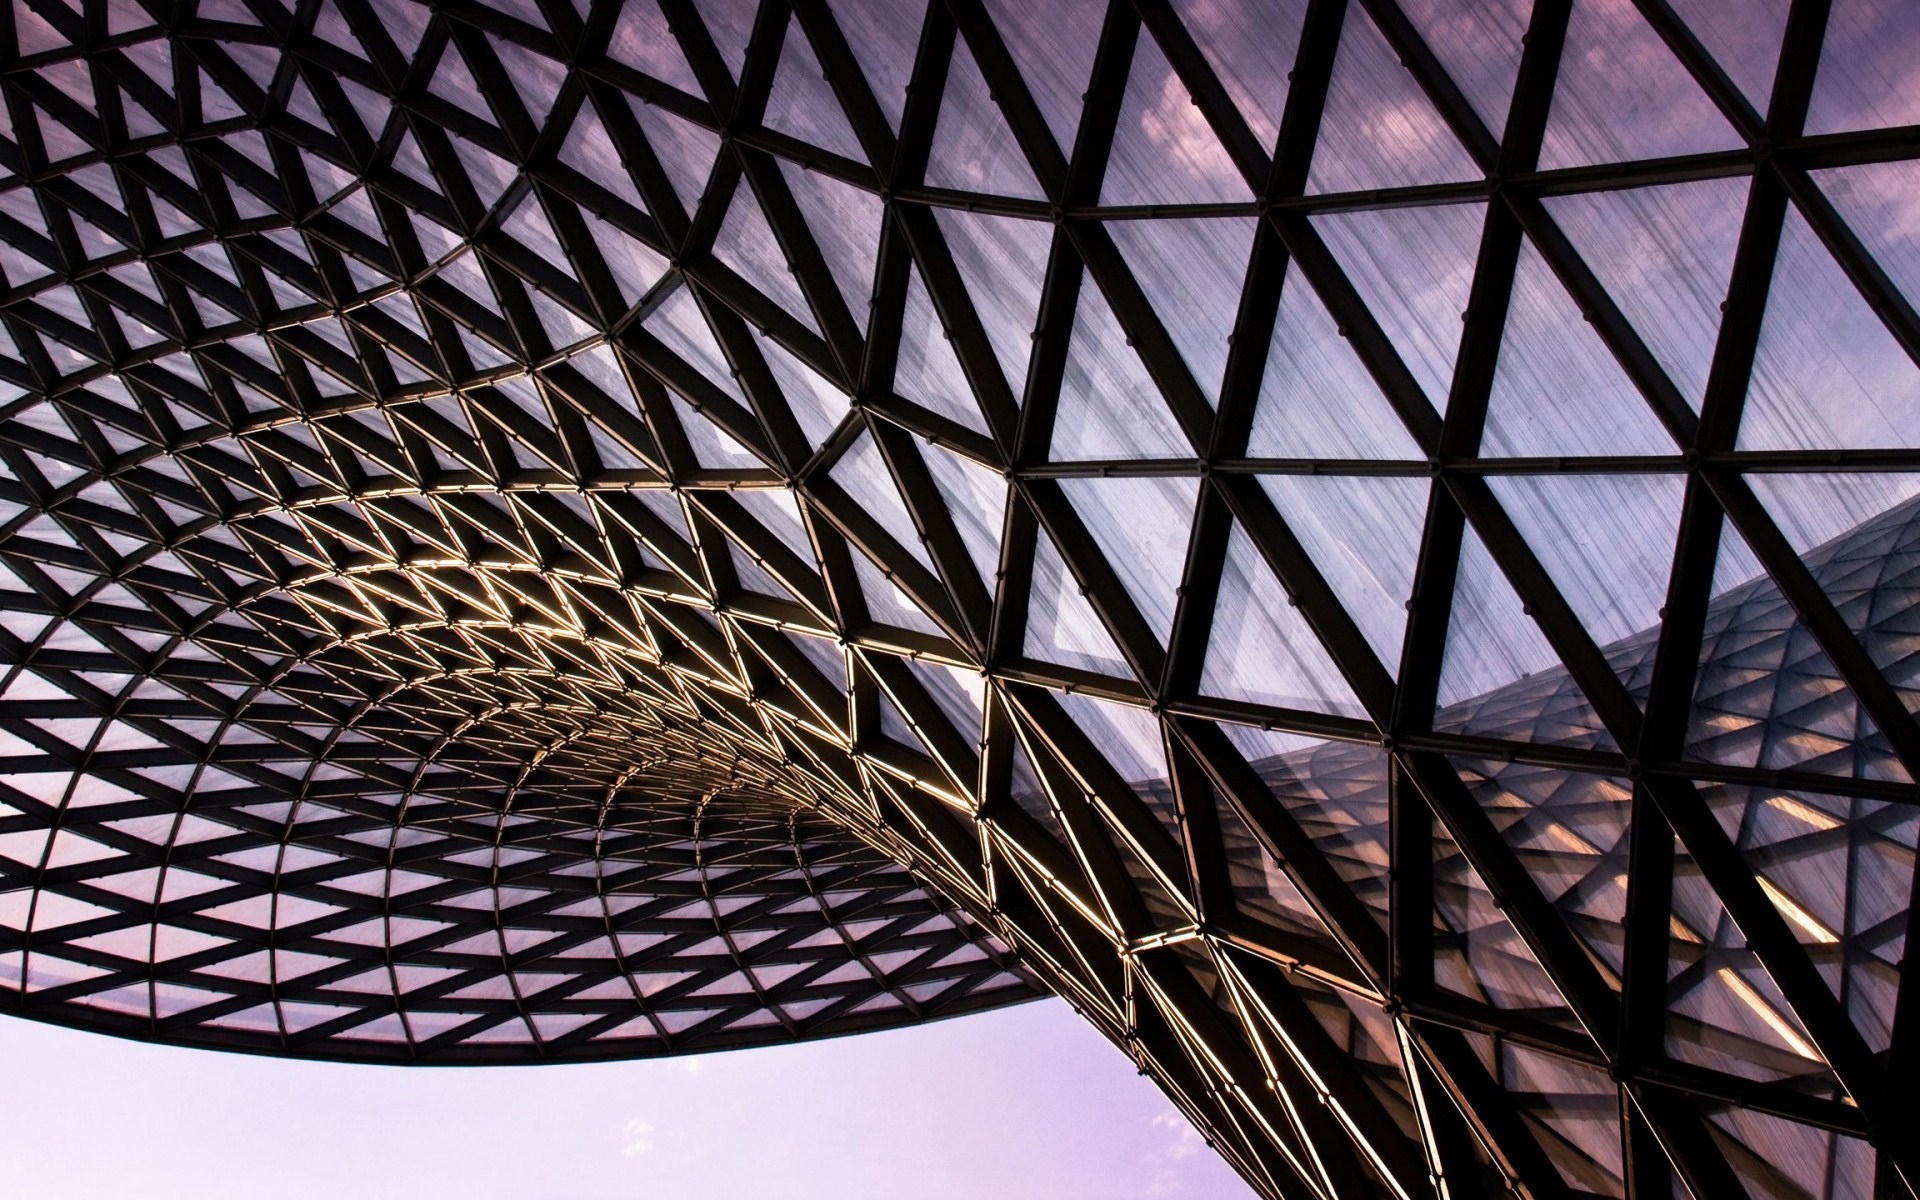
\includegraphics[width=5in]{structure} \\[1cm] % Figura del trabajo -Se puede comentar y dejar el espacio en blanco si se quisiera.
	% Autores y docentes
	
	\vspace{-0.5cm}
	
	\noindent
	\begin{flushleft} \large
		\emph{Autores:}\\
		Nombre \textsc{Apellido} - C.I.: X.XXX.XXX-X \\
		Nombre \textsc{Apellido} - C.I.: X.XXX.XXX-X \\
		Nombre \textsc{Apellido} - C.I.: X.XXX.XXX-X \\
		Nombre \textsc{Apellido} - C.I.: X.XXX.XXX-X \\
		
		\vspace{0.5cm}
		
		\emph{Docentes:} \\
		Nombre \textsc{Apellido}\\
		Nombre \textsc{Apellido}\\
		Nombre \textsc{Apellido}
	\end{flushleft}
	\vfill
	
	% Fecha
	{\large \today}
	
	\end{center}
\end{titlepage}

\thispagestyle{empty} % Para que no aparezca numero de pagina
\newpage              % Salta a nueva página


\tableofcontents      % Crea índice (o tabla de contenidos). Hay que compilar 2 veces para que se actualice.
\thispagestyle{empty} % Para que no aparezca numero de pagina en esta carilla.
\newpage              % Se usa \newpage al final para que no ajuste todo el índice al tamaño de la hoja

\clearpage

\pagenumbering{arabic} % Define el tipo de numeración de las páginas.

\section{Trabajando con \LaTeX}
\subsection{Introducción}
	
	En este documento se explican la gran mayoría de las cosas simples y básicas para hacer en \LaTeX. Luego al crear su propio documento el usuario puede copiar el código de este template y modificar los datos para usarlo con otro fin. 
	
	Este template es de libre distribución y se puede modificar según lo que uno necesite. En lo que sigue se va a explicar como escribir dentro de \LaTeX, por lo que luego de compilar uno puede volver al código y entender como se escribió el código. Vale aclarar que hay varias formas para lograr lo mismo, por lo que posiblemente hayan mejores o peores formas de escribir ciertas expresiones. Ésto aplica para todo en \LaTeX, desde como expresar una fórmula matemática, a colocar figuras o presentar una tabla.

\subsection{Editando texto}
	Hay diferentes tipos de \textit{Font Styles}, puedo tener palabras en \textbf{negrita} o en \textit{itálica} como también \underline{subrayadas}, se puede poner \emph{énfasis} o escribir \textsl{inclinado}. Está el estilo \texttt{máquina de escribir}, el de \textsc{pequeña capitalización} o sino \textsf{Sans Serif}.
	
	Respecto al tamaño de texto de alguna palabra, frase o párrafo, puedo escribir {\tiny super chiquito}, no tan {\scriptsize chiquito}, un poquito menos {\footnotesize chico}, un poco menos {\small chico}. Sino puedo escribir un poco más {\large grande}, otro poco más {\Large grande}, bastante {\LARGE grandioso}, sino {\huge gigante } y hasta {\Huge gigantesco}. Lo bueno de esto es que los tamaños de letra están relacionados por adjetivos respecto al tamaño de letra determinado al definir el tipo de clase de documento, por lo que si se llegara a cambiar, por ejemplo, de 12pt a 11pt, el tamaño de todos los textos del documento se ajustaría proporcionalmente, manteniendo la misma armonía de antes.
	
	Al trabajar con texto, para indicar que quiero hacer un punto y aparte, simplemente hay que escribir una línea y luego dejar otra en blanco, de esa forma \LaTeX ~entiende que tiene que hacer un punto y aparte. 


	Al hacer el punto y aparte de esta forma, la sangría se agrega automáticamente. Si se quiere indicar un salto de línea se puede escribir \verb|\\| y se sigue en la otra y no va a tener sangría la línea siguiente. Para forzar sangría se pone \verb|\indent| y para forzar que no haya \verb|\noindent|. Luego de una imagen o tabla se agrega sangría automáticamente. Otra forma de generar espacio vertical es con el comando \verb|\vspace{length}| donde \verb|length| puede por ejemplo ser 1.32cm.
	
	\vspace{1.32cm}
	
	Se coloca ahora un salto de página con el comando \verb|\newpage|.
	
	\newpage
	

\subsection{Trabajando con imágenes}

	Se ejemplifica a continuación una imagen puesta normalmente (TeXstudio, en menú \textit{Wizards} $ \Longrightarrow $ \textit{Insert Graphic...}, contiene una interfaz gráfica para facilitar la colocación de imágenes.). Se debe referenciar cada figura que uno coloca dentro del texto, así uno sabe que en la \autoref{fig:sim}  hay algo relacionado a lo que estoy hablando.
	\begin{figure}[h!]
	\centering
	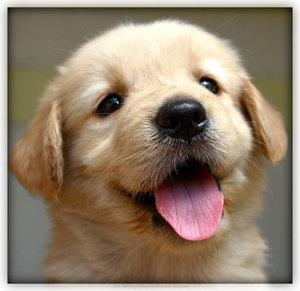
\includegraphics[width=.3\textwidth]{puppy}
	\caption{Caption de la figura describiendo que tiene la misma.}
	\label{fig:sim}
	\end{figure}
	
	También se puede poner dos subfiguras dentro de la definición de una figura (\autoref{fig:doble}), lo cual puede ser útil para hablar de dos gráficas relacionadas o algo similar. 
	\begin{figure}[h!]
	\centering
	\subfloat[Caption de subfigura 1.]{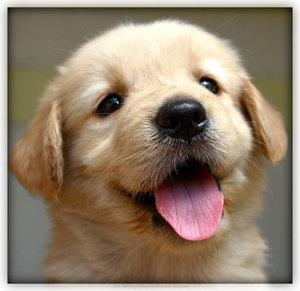
\includegraphics[width=1.7in]{puppy}%
	\label{fig_first_case}} 
	\hfil
	\subfloat[Caption de subfigura 2.]{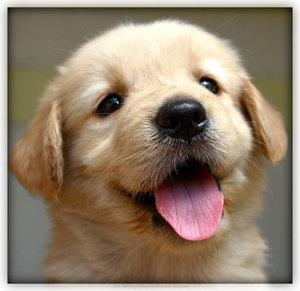
\includegraphics[width=1.7in]{puppy}%
	\label{fig_second_case}}
	\caption{Este es un caso en donde se pueden poner dos imágenes juntas, se tiene la \autoref{fig_first_case} y por otro lado se tiene la \autoref{fig_second_case}.}
	\label{fig:doble}
	\end{figure}
	
	\newpage %% Salto de página
	
	\begin{wrapfigure}[13]{r}{0.4\textwidth} %% [11] indica cantidad de lineas de texto a utilizar para la imagen. Si se elimina se calcula automáticamente.
		\begin{center}
			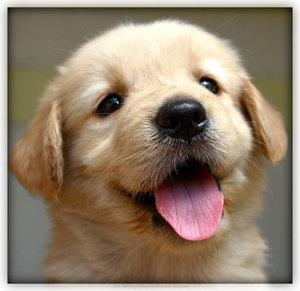
\includegraphics[width=1.7in]{puppy}
		\end{center}
		\caption{Un cachorro.} \label{fig:cachorro}
	\end{wrapfigure}
	% Notar que el texto a colocar al lado de la figura debe estar debajo del entorno wrapfigure
	Puede ser útil utilizar el entorno \verb|wrapfigure| para colocar una imagen al lado de texto, como es el caso de la \autoref{fig:cachorro}. Este texto puede contener lo que sea, como tablas o ecuaciones, simplemente lo que sucede es que el ancho de linea se reduce por la imagen, nada más.
		
	
	Hay más opciones de como mostrar figuras, por ejemplo que estén dentro de un párrafo o que su \verb|caption| esté al costado y no abajo\footnote{Ver más en \url{http://en.wikibooks.org/wiki/LaTeX/Floats,_Figures_and_Captions}}.  
	
	Puede ser útil utilizar el paquete \verb|overpic|, el cual permite colocar texto o ecuaciones sobre imágenes que tengamos. Esto es de gran utilidad para crear documentos de elevada calidad y presentación. Por ejemplo, en la \autoref{fig:neopreno} se tienen las variables $ \mathbf{t} $ y $ \mathbf{e} $ y en la imagen las variables que aparecen son las \underline{mismas}, en tamaño y formato, facilitando la lectura e interpretación entre el texto y las figuras que aparecen. 
	
	Se puede colocar texto como ecuaciones, con cualquier formato e inclinación.
	
	\begin{figure}[h!]
		\centering
		\begin{overpic}[width=0.6\textwidth,tics=5]{Neopreno} % Poner ",grid" luego de tics para activar la grilla. "tics" es la separación en la grilla.
			\put (07,20) { $ \mathbf{t} $}
			\put (07,15) { $ \mathbf{t} $}
			\put (88,22) { $ \mathbf{e} $}
			\put (88,16) { $ \mathbf{e} $}
			\put (88,11) { $ \mathbf{e} $}
			\put (17,63) {\rotatebox{30}{$ \mathbf{a} $}}
			\put (50,67) {\rotatebox{-30}{$ \mathbf{b} $}}
			\put (16,13) {\rotatebox{30}{2.5}}
			\put (16,30) {\rotatebox{30}{2.5}}
			\put (31,49) {\rotatebox{30}{2.5}}
			\put (56,48) {\rotatebox{-28}{2.5}}
			\put (63,67) {Chapas de acero}
			\put (05,08) {Elastómero}
		\end{overpic}
		\caption{Composición de un apoyo elastomérico.}
		\label{fig:neopreno}
	\end{figure}	
	
Para editar y generar imágenes de alta calidad puede ser útil el programa \href{https://inkscape.org/es/}{Inkscape}\footnote{Inkscape: \url{https://inkscape.org/es/}}. Otro programa que puede ser útil para la edición es \href{https://www.gimp.org/}{GIMP}\footnote{GIMP: \url{https://www.gimp.org/}}. Ambos programas son gratuitos.

\subsection{Diferentes listas}

	Tenemos varias formas de hacer listados en \LaTeX. Por ejemplo se puede hacer una lista con cuadrados negros utilizando el entorno \verb|itemize|
	\begin{itemize}
	\item Se pone un ítem
	\item Y se puede seguir poniendo hasta donde uno quiera
	\item Se escribe \verb|\item| para agregar otro punto 
	\item Tocando Ctrl+Shift+I agrega otro ítem automáticamente
	\end{itemize}
	
	Se puede hacer una lista numerada utilizando el entorno \verb|enumerate|
	\begin{enumerate}
	\item Primer ítem
	\item Se aplica lo mismo explicado anteriormente
	\end{enumerate}
	
	Otro tipo de lista muy útil es la llamada \verb|description| en la cual se pueden definir varios conceptos de manera prolija
	\begin{description}
	\item[Palabra] Explico lo que quiera de la \textit{palabra} que estoy definiendo o describiendo.
	\item[Otra cosa] Y así puedo seguir al igual que en los otros entornos.
	\item[Definición larga] Cuando tengo mucho para decir de algo, el texto en las líneas siguientes se ajusta de forma diferente a los párrafos usuales para que se note que uno está dentro de este entorno de descripción y que se refiere a la palabra en negrita.
	\end{description}
	
\subsection{Utilizando ecuaciones}
	
	En esta sección vamos a ver algunas formas básicas de como insertar ecuaciones y lenguaje matemático dentro del documento. Para escribir algo en lenguaje matemático dentro de la línea de texto se lo encierra entre los signos de \$. Si no se hace esto la fórmula escrita va a dar error. Entonces escribir \verb|$F=mg\cos(\theta)$| genera la ecuación $F=mg\cos(\theta)$. Para escribir una fórmula en la siguiente línea y centrada se encierra la misma con dos \$, entonces \verb|$$F=mg\cos(\theta)$$| genera
	$$F=mg\cos(\theta)$$
	aunque esto es medio ``desprolijo''. Es mejor trabajar con el entorno \verb|equation|, el cual tiene la siguiente sintaxis:
	\begin{verbatim}
	\begin{equation}
	content...
	\end{equation}
	\end{verbatim}
	Todo lo que se escriba donde dice \verb|content...| estará en lenguaje matemático y no necesita signos de \$ (de ponerse \$ hay error). Al usar este entorno la ecuación queda numerada, lo cual es lo usual. Este template numera las ecuaciones por sección y reinicia el conteo en cada una. Por lo tanto una ecuación se vería así
	\begin{equation}\label{eq:1}
	E=mc^2
	\end{equation}
	Además de estar numerada también se puede referenciar y hablar de la Eq. \eqref{eq:1}. Si no se quiere que la ecuación esté numerada se agrega un * al definir la ecuación, es decir: \verb|equation*|. Sería lo siguiente:
	\begin{equation*}
	E=mc^2
	\end{equation*}
	Se puede escribir texto dentro de una ecuación utilizando dentro del entorno matemático \verb|\text{texto}|, por ejemplo:
	\begin{equation}\label{eq:2}
	F=mg\cos(\theta) ~ \text{texto.}
	\end{equation}
	En este caso se escribe texto y se pone en negrita también
	\begin{equation}
	\textbf{K}^{(e)}\textbf{a}^{(e)} - \textbf{f}^{(e)} = \textbf{q}^{(e)}
	\end{equation}
	El superíndice y el subíndice se escriben asi:
	\begin{equation}
	e^{x} \quad f_{yk} \quad R_{n}^{i+1}
	\end{equation}
	
	Utilizando el comando \verb|\,| se genera un espacio. Utilizando \verb|\quad| o \verb|\qquad| se generan espacios mayores. También se pueden setear distancias horizontales genéricas con \verb|\hspace{length}|.\\
	
	Puedo escribir integrales, sumatorias y fracciones de esta forma:
	\begin{equation}
	\int_{0}^{\infty}\frac{\partial Q_{y}}{\partial y}\,\text{d}\,y \qquad \sum_{i=1}^{n}i^2.
	\end{equation}
	Combinando todo lo anterior
	\begin{equation}
	\int_{l^{(e)}} \delta\kappa Mdx = \int_{l^{(e)}} \left( \delta \omega f_z + \delta\left( \frac{\partial\omega}{\partial x}\right) m  \right) dx + \sum_{i=1}^{2} \left[ \delta\omega_i F_{z_i} + \delta \left( \frac{\partial\omega}{\partial x}_i\right) M_i \right].
	\end{equation}
	Lo importante es ser ordenado y asegurarse que todo cierre para no tener errores al compilar
	\begin{equation}
	\left( \int_{-1}^{+1} \textbf{B}_b^T \textbf{B}_b \frac{EI_y l^{(e)}}{2}d\xi\right)\text{\textbf{a}}^{(e)} - \int_{-1}^{+1} (\text{N}^T f_x + \hat{\text{N}}^T m) \frac{l^{(e)}}{2}d\xi = \text{\textbf{q}}^{(e)}
	\end{equation}

\subsection{Matrices y tablas}
	 Si quiero escribir matrices, arrays, o algo similar lo más cómodo y simple es ir a: \textit{Wizards$\mapsto$Quick Array.} y ahí elegir la cantidad de columnas, filas, posición en cada celda y el tipo de environment. Tienen que estar dentro de una \verb|equation| para poder compilar o entre los signos \$\$. Un \verb|array| y una \verb|matrix| tiene diferente forma de trabajo, a los \verb|array| hay que especificar la cantidad de columnas, mientras que con una \verb|matrix| no. A modo de ejemplo, esto es un array centrado:
	\begin{equation*}
	\begin{array}{cccc}
	38 & \frac{EI}{L} & 2144 & GA\\ 
	a+b & \varepsilon & &
	\end{array} 
	\end{equation*}
	Esto es un array cambiando la alineación y agregando paréntesis
	\begin{equation*}
	\left( \begin{array}{rclc}
	38 & \frac{EI}{L} & 2144 & GA\\ 
	a+b & \varepsilon & &
	\end{array} \right) 
	\end{equation*}
	\begin{equation*}
	\left[  \begin{array}{rclc}
	38 & \frac{EI}{L} & 2144 & GA\\ 
	a+b & \varepsilon & &
	\end{array} \right]  
	\end{equation*}
	\begin{equation*}
	\left\lbrace  \begin{array}{rclc}
	38 & \frac{EI}{L} & 2144 & GA\\ 
	a+b & \varepsilon & &
	\end{array} \right\rbrace  
	\end{equation*}
	Todas las \verb|matrix| como \verb|array| están dentro de un entorno matemático por lo que no hay que usar el símbolo de \$. Esto no es así al trabajar con tablas. De la misma manera, lo más fácil para insertar una tabla es a través del \textit{Wizard} del editor de texto. Una tabla común se define dentro del entorno $\backslash$tabular. Esta es bastante limitada y se debe especificar donde colocarla. Se puede colocar dentro de la línea, en la siguiente y orientarla hacia un lado u otro como si fuese un párrafo de texto.
	\begin{center}
	\begin{tabular}{|c|c|c|c|}
	\hline   & 1 & 2 & 3 \\ 
	\hline A &  &  &  \\ 
	\hline B &  &  &  \\ 
	\hline 
	\end{tabular} 
	\end{center}
	En cada entrada, si se quiere poner algún símbolo matemático, hay que usar los símbolos de \$. Es preferible definir la tabla dentro del entorno \verb|\table|. De esta forma uno puede referenciar la \autoref{tab:ejemplo}, ésta va a estar numerada y tener caption. 
	\begin{table}[h!]
	\renewcommand{\arraystretch}{1.3} % Hace filas más altas para  que entre la fracción
	\caption{Título de la tabla}
	\label{tab:ejemplo}
	\centering
	\begin{tabular}{|r|l|}
	  \hline
	  7C0 & hexadecimal \\
	  3700 & octal \\ \cline{2-2} %linea horizontal solo en la columna 2
	  11111000000 & binary \\
	  \hline \hline
	  1984 & decimal \\
	  \hline
	\end{tabular}
	\end{table}
	
	
También se puede poner dos subtablas dentro de la definición de una tabla (\autoref{tab:subtablas}), como se ve a continuación. La sintaxis es similar a la de subfiguras.
\begin{table}[h!]
	\centering
	\caption{Resultados experimentales} \label{tab:subtablas}
	\subfloat[Tensión]{%
		\begin{tabular}{|c|r|r|r|}
			\hline
			A       & B   & C    & D\\
			\hline
			\hline
			a       & a  & c    & d\\
			\hline
		\end{tabular}%
	}\hspace{1cm} %% Separación entre subtablas
	\subfloat[Deformación]{%
		\begin{tabular}{|c|r|r|r|}
			\hline
			A       & B   & C    & D\\
			\hline
			\hline
			a       & a  & c    & d\\
			\hline
		\end{tabular}}
	\end{table}

	Se puede ver la versatilidad al editar la tabla, definiendo líneas, colocando fracciones, etc.. Por ejemplo en la IEEE solo usan lineas horizontales para sus tablas, ver \autoref{tab:IEEE}.
	\begin{table}[h!]
	\renewcommand{\arraystretch}{1.3}
	\caption{Tablas estilo IEEE}
	\label{tab:IEEE}
	\centering
	\begin{tabular}{c c c }
	\hline
	 & Largo & Ancho \\
	\hline
	Sección 1 & 15 cm & 5 cm\\
	Sección 2 & 10 cm & 5 cm\\
	\end{tabular}
	\end{table}

	
	Por ejemplo si quiero poner texto, puedo especificar el ancho total de una columna y que el texto se ajuste a dicho ancho, ver \autoref{tab:aux}.
	\begin{table}[h!]
		\renewcommand{\arraystretch}{1.3}
		\caption{Tablas estilo IEEE}
		\label{tab:aux}
		\centering
		\begin{tabular}{ | l | l | l | p{5cm} |}
			\hline
			Day & Min Temp & Max Temp & Summary \\ \hline
			Monday & 11C & 22C & A clear day with lots of sunshine.  
			However, the strong breeze will bring down the temperatures. \\ \hline
			Tuesday & 9C & 19C & Cloudy with rain, across many northern regions. Clear spells
			across most of Scotland and Northern Ireland,
			but rain reaching the far northwest. \\ 
			\hline
		\end{tabular}
	\end{table}

\newpage

	Es útil también saber como tener filas o columnas que abarquen varias columnas o filas respectivamente\footnote{Más ejemplos en \url{http://en.wikibooks.org/wiki/LaTeX/Tables}}, ver \autoref{tab:aux2}.
	
	\begin{table}[h!]
		\renewcommand{\arraystretch}{1.3}
		\caption{Tablas estilo IEEE}
		\label{tab:aux2}
		\centering
		\begin{tabular}{ |l|l|l| } % 3 columnas con orientación hacia la izquierda
			\hline
			\multicolumn{3}{ |c| }{Team sheet} \\ %solo esta fila es una columna sola
			\hline
			Goalkeeper & GK & Paul Robinson \\ \hline
			\multirow{4}{*}{Defenders}   & LB & Lucus Radebe \\
			& DC & Michael Duburry \\
			& DC & Dominic Matteo \\
			& RB & Didier Domi \\ \hline
			\multirow{3}{*}{Midfielders} & MC & David Batty \\
			& MC & Eirik Bakke \\
			& MC & Jody Morris \\ \hline
			Forward                      & FW & Jamie McMaster \\ \hline
			\multirow{2}{*}{Strikers}    & ST & Alan Smith \\
			& ST & Mark Viduka \\
			\hline
		\end{tabular}
	\end{table}
	

\newpage % Crea una nuevz página, recomendable antes de cada sección

\section{Matemática avanzada}
\subsection{Combinando varias herramientas}
	Una vez que uno tiene que empezar a escribir informes más detallados, en donde necesita mostrar ecuaciones o fórmulas más complicadas de escribir, a veces es útil utilizar paquetes que resuelvan de manera más eficiente ciertas situaciones o simplemente combinar varias herramientas de \LaTeX. Por ejemplo, si uno quiere hacer una lista de diferentes cálculos, puede combinar el entorno \verb|enumerate| con \verb|equation|. Si una ecuación es muy larga, se puede utilizar el entorno \verb|multiline| el cual permite escribir ecuaciones en varias líneas.
	
	\begin{enumerate}
	\item Equilibrio vertical:
	\begin{multline*}
	pRd\varphi-Q_r\cos\left(\frac{d\varphi}{2}\right)+(Q_r+dQ_r)\cos\left(\frac{d\varphi}{2}\right) \qquad\\
	+N_\varphi \sen\left(\frac{d\varphi}{2}\right)+(N_\varphi+dN_\varphi)\sen\left(\frac{d\varphi}{2}\right)=0
	\end{multline*}
	\begin{equation}\label{eq:mult1}
	\Rightarrow \boxed{pRd\varphi+dQ_r+N_\varphi d\varphi=0}
		\end{equation}
	%
	\item Equilibrio horizontal:
	\begin{multline*}
	qRd\varphi-Q_r\sen\left(\frac{d\varphi}{2}\right)-(Q_r+dQ_r)\sen\left(\frac{d\varphi}{2}\right) \qquad \\
	-N_\varphi \cos\left(\frac{d\varphi}{2}\right)+(N_\varphi+dN_\varphi)\cos\left(\frac{d\varphi}{2}\right)=0
	\end{multline*}
	\begin{equation}\label{eq:mult2}
	\Rightarrow \boxed{qRd\varphi-Q_rd\varphi+dN_\varphi=0}
		\end{equation}
	%
	\item Sumatoria de los momentos respectos de $O$:
	\begin{equation*}
	\qquad \qquad \quad qR^2d\varphi-N_\varphi R+(N_\varphi+dN_\varphi)R -M_z+(M_z+dM_z)=0
	\end{equation*}
	\begin{equation}\label{eq:mult3}
	\Rightarrow \boxed{qR^2d\varphi+dN_\varphi R + dM_z=0}
	\end{equation}
	\end{enumerate}
	Se utilizó el comando \verb|boxed| para encuadrar una ecuación. Otra posibilidad útil es poder escribir varias ecuaciones alineadas, así sea como una resolución de operaciones como para presentar varias ecuaciones. Para eso se usa el entorno \verb|align|.
	\begin{align}
	x&=a \text{Arcsenh}\left(\tan(\alpha) \right) \\
	y&=\frac{a}{\cos(\alpha)-1}
	\end{align}
	También se puede utilizar sin que numere las ecuaciones o que numere solo una.
	\begin{align}
	x & = (a+b)^2 \nonumber \\
	  & = (a+b)\times (a+b) \nonumber \\
	  & = a^2+2ab+b^2 
	\end{align}
	
	Otra forma de hacer lo anterior es utilizar el entorno \verb|eqnarray| en sustitución de \verb|align|.\\
	
	Un problema que puede suceder es que una ecuación que queramos encuadrar sea muy larga y ocupe varias líneas. Ahí el comando \verb|boxed| no funciona y una opción es utilizar el entorno \verb|empheq| el cual combina el comando \verb|align| con \verb|boxed|, entre otros, permitiendo escribir algo de este estilo:
	\begin{empheq}[box=\fbox]{align}
	\begin{split}
	Q_r(\alpha)=&\frac{\gamma \text{tan}(\alpha)}{2a}-\frac{\gamma \text{cos}(\alpha)\text{log}(\text{cos}(\alpha /2)-\text{sen}(\alpha /2))}{2a} \\
	 &+ \frac{\gamma \text{cos}(\alpha)\text{log}(\text{sen}(\alpha /2)+\text{cos}(\alpha /2))}{2a}+ C_1 \text{sen}(\alpha)+ C_2 \text{cos}(\alpha)
	\label{eq:cortante_catenaria}
	\end{split}
	\end{empheq}
	
	Si queremos enumerar las ecuaciones como sub-ecuaciones se puede por ejemplo utilizar el entorno \verb|subecuations|. Las ecuaciones de Maxwell son:
	\begin{subequations}
		\begin{align}
	        B'&=-\nabla \times E,\\
	        E'&=\nabla \times B - 4\pi j,
	\end{align}
	\end{subequations}
	Es útil también hacer comentarios en ecuaciones o indicar algo en especial, esto es una forma:
	\begin{equation}
	 z = \overbrace{
	   \underbrace{x}_{\text{Re}(z)} + i\underbrace{y}_{\text{Im}(z)}
	  }^\text{Número complejo},
	\quad 
	 y = a + f(\underbrace{b x}_{
	                    \ge 0})
	\end{equation}
	Si quiero escribir funciones discontinuas lo puedo hacer de esta forma:
	\begin{equation}
	u(x) =
	  \begin{cases}
	   e^{x} & \text{if } x \geq 0 \\
	   1       & \text{if } x < 0
	  \end{cases}
	\end{equation}
	Si se combinan varias formas vistas anteriormente se puede escribir algo de este estilo:
	\begin{equation}
\text{Ecuaciones de Maxwell:}\,\,\begin{cases}
B'&=-\nabla \times E,\\
E'&=\nabla \times B - 4\pi j.
\end{cases}
	\end{equation}
	Hay más información respecto a formas avanzadas de trabajar en lenguaje matemático al que le interese\footnote{Ver más en \url{http://en.wikibooks.org/wiki/LaTeX/Advanced_Mathematics}}.

\newpage 

% Ejemplos de referencias escritas de la forma más simple en LaTeX. Se podría generar y luego importar un archivo .bib si uno quisiera.

\section{Bibliografía}


Es usual en el texto referenciar la bibliografía utilizada. Por ejemplo, un libro se cita con \verb|\cite{label}| donde \verb|label| es la etiqueta de la citación. El libro \textit{Structural Analysis with The Finite Element Method-Linear Statics, Vol. 2: Plates and Shells} se cita como \cite{Onate}. Luego las otras dos referencias se pueden citar juntas como \cite{Lenci,Zienkiewicz}.


\bibliographystyle{plain}



\begin{thebibliography}{5} %
\thispagestyle{empty}
%
\bibitem{Lenci}
Lenci, S. y Clementi, F. \emph{Simple Mechanical Model of Curved Beams by a 3D Approach.} \relax Journal of Engineering Mechanics, ASCE, 2009.
%
\bibitem{Onate}
Oñate, E. \emph{Structural Analysis with The Finite Element Method-Linear Statics,
Vol. 2: Plates and Shells} 1st~ed. \relax Springer-CIMNE, 2013.
%
\bibitem{Zienkiewicz}
Zienkiewicz, O.C. y Taylor, R.L. \emph{El método de los elementos finitos. Vol. 2: Mecánica de sólidos y fluidos. Dinámica y no linealidad.} 6ta~ed. \relax Elsevier, 2005.
%
\end{thebibliography}





\end{document}